\newpage

\customsection{Реализация фильтрационного слоя новостей}

\customsubsection{Обоснование выбора технологий}
Выбор технологий для реализации системы мониторинга новостных ресурсов и, в частности, фильтрационного слоя, базируется на результатах анализа, представленного в главе 1.
В рамках анализа были выделены ключевые требования к системе: поддержка масштабируемой микросервисной архитектуры, обеспечение отказоустойчивости, высокая наблюдаемость, а также применение современных методов фильтрации контента, включая дедупликацию, анализ тональности и оценку потенциальной вирусности.
\begin{itemize}
    \item \textbf{Микросервисный подход} в совместной работе был выбран как базовая архитектурная парадигма ввиду его соответствия принципам отказоустойчивости и масштабируемости (см.\ п. ~\ref{subsec:anal12}).
    Он позволяет изолировать критически важные компоненты, упростить развертывание и ускорить развитие системы.
    \item В качестве \textbf{инструмента оркестрации контейнеров} выбран \textbf{Docker Swarm}.
    Это решение обеспечивает автоматизированное развертывание и поддержку отказоустойчивых сценариев при сбоях отдельных сервисов.
    \item Для \textbf{фильтрации контента} реализован ряд механизмов, описанных в разделе 1.1: дедупликация на основе семантического сходства (см.\ п. ~\ref{subsubsec:anal111}), фильтрация по ключевым словам (см.\ п. ~\ref{subsubsec:anal112}), анализ тональности с использованием предобученной модели для русского языка (см.\ п. ~\ref{subsubsec:anal113}), а также вычисление вирусности с применением batched inference через REST API (см.\ п. ~\ref{subsubsec:anal114}).
    \item Для \textbf{сбора логов и телеметрии} выбрано решение на базе \textbf{Filebeat} + \textbf{Elasticsearch} + \textbf{Kibana} (см.\ п. ~\ref{subsec:anal13}), обеспечивающее полную наблюдаемость за всеми компонентами системы, включая анализ ошибок, метрик загрузки и отслеживание состояния очередей.
    \item Во всех синхронных взаимодействиях между микросервисами реализована \textbf{политика повторных попыток (retry policy)}, что соответствует рекомендациям по построению отказоустойчивых распределённых систем и снижает вероятность потери данных при кратковременных сбоях (см.\ п. ~\ref{subsec:anal12}).
\end{itemize}

Таким образом, выбранный стек технологий и архитектурные решения напрямую опираются на выявленные в исследовании требования к системе, а также соответствуют современным промышленным практикам построения отказоустойчивых и интеллектуальных систем обработки данных.

\customsubsection{Общая архитектура системы мониторинга новостей}
Разрабатываемая система мониторинга новостей построена на основе микросервисной архитектуры, в которой каждый компонент отвечает за строго определённую функцию в процессе обработки новостного потока.
Основу взаимодействия между компонентами составляет асинхронная коммуникация через брокер сообщений \textbf{RabbitMQ}, а для хранения данных используется \textbf{MongoDB} и \textbf{Elasticsearch}.

\begin{figure}[H]
    \centering
    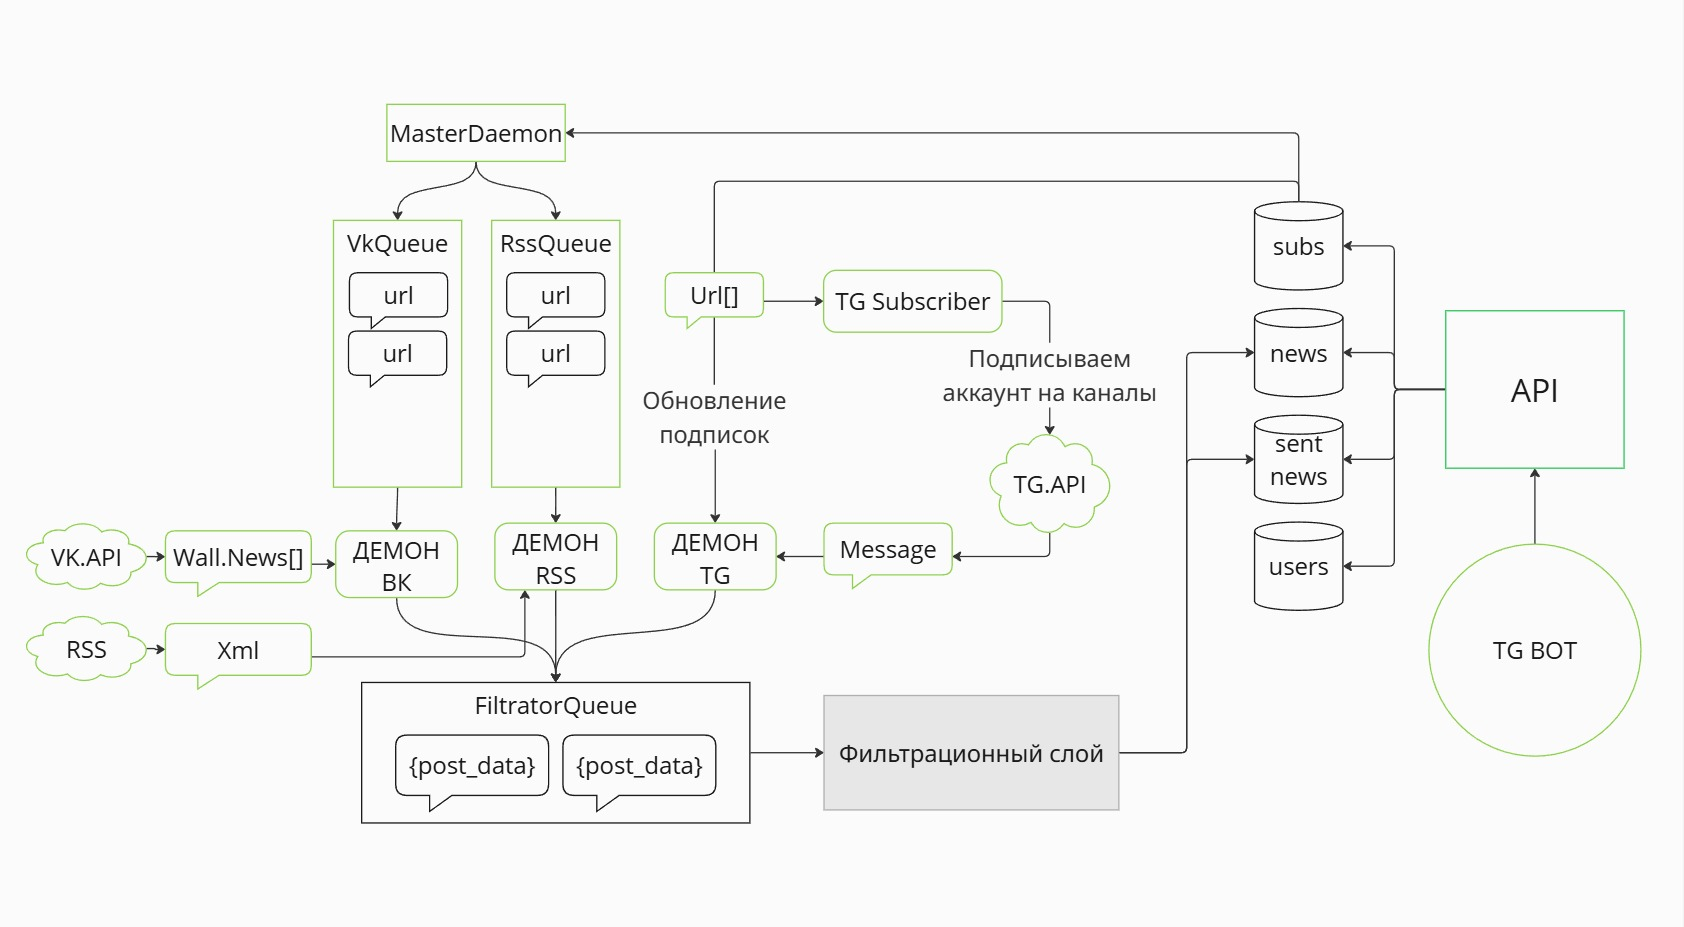
\includegraphics[width=150mm]{images/all_process}
    \caption{Общая архитектура системы мониторинга новостей, рассмотренная в данной работе}
    \label{fig:all_process}
\end{figure}

На входе системы работают демоны-парсеры, ответственные за сбор новостной информации из различных источников: \textbf{социальных сетей} (VK, Telegram) и \textbf{RSS-лент}.
Каждый демон осуществляет непрерывный мониторинг доверенных источников, извлекает новые публикации и помещает их в очередь сообщений \texttt{filtration}.
Эти демоны разрабатывались параллельно с данной работой и в её рамках не рассматривались детально, однако их функциональность важна для полноценного функционирования всей системы.

Следующим этапом обработки является \textbf{фильтрационный слой}, который принимает на вход собранные новости и выполняет интеллектуальную фильтрацию, включая анализ содержания и пользовательские предпочтения.
Результаты работы фильтрационного слоя сохраняются в базе данных и формируют коллекцию новостей, готовых к отправке пользователям.

Последняя стадия обработки — \textbf{доставка новостей конечным пользователям}, которая реализуется с помощью \textbf{Telegram-бота}.
Бот периодически запрашивает через Web Api подготовленные сообщения из коллекции \texttt{NewsToSend} и отправляет их в соответствующие каналы или личные чаты в Telegram.
Отправка производится с учётом индивидуальных настроек пользователей, включая предпочтения по тематикам, ключевым словам и режиму уведомлений.

\customsubsection{Архитектура фильтрационного слоя}\label{subsec:filtersloy}
Фильтрационный слой системы мониторинга новостей реализован как связка специализированных микросервисов, объединённых единой очередью сообщений и REST-интерфейсами для вызова вспомогательных компонентов.
Основной задачей фильтрационного слоя является интеллектуальная обработка новостных сообщений: от базовой предобработки до персонализированной фильтрации под конкретных пользователей.

\begin{figure}[H]
    \centering
    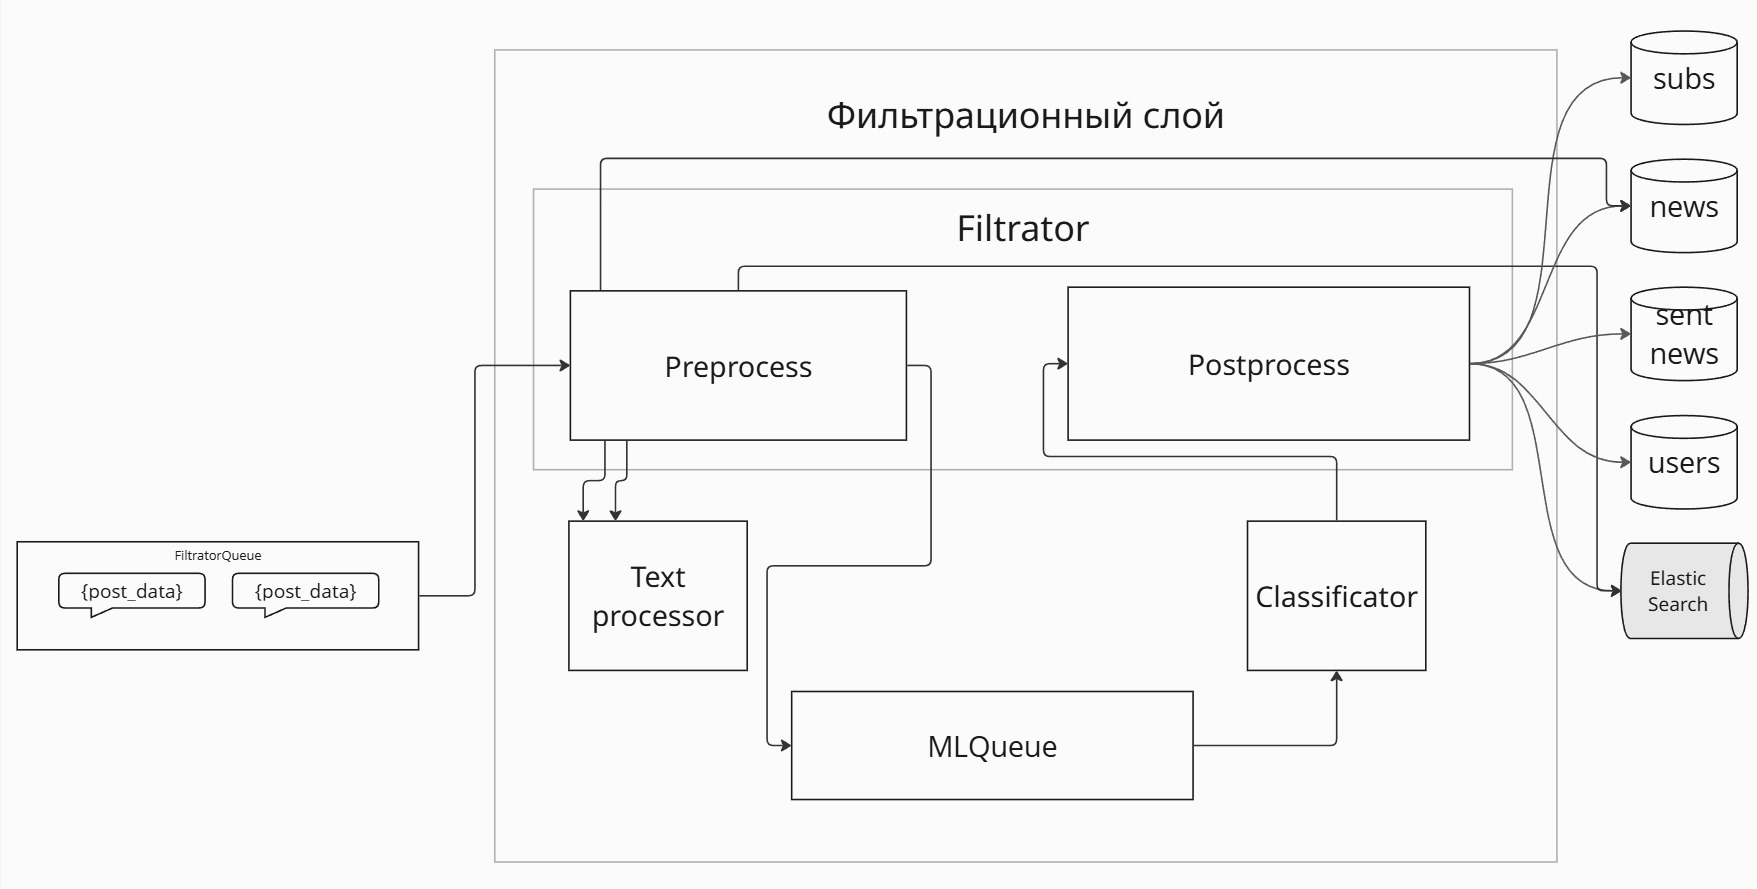
\includegraphics[width=150mm]{images/filter_process}
    \caption{Общая архитектура системы мониторинга новостей, рассмотренная в данной работе}
    \label{fig:filter_process}
\end{figure}

Центральным элементом слоя является микросервис \textbf{Filtrator}, реализующий цепочку обработки новостей.
Архитектурно он организован вокруг следующих компонентов и взаимодействий:
\begin{itemize}
    \item \textbf{Очередь входящих сообщений (filtration)} — источник входных данных, поступающих от демонов парсинга.
    Filtrator подписывается на неё и обрабатывает каждое сообщение независимо, используя пул воркеров.
    \item \textbf{Предобработка сообщений} включает:
    \begin{itemize}
        \item проверку времени и корректности формата данных;
        \item дедупликацию по ID;
        \item векторизацию текста через вызов сервиса TextProcessor;
        \item анализ тональности, также с использованием TextProcessor;
        \item определение смысловых дубликатов с помощью векторного сравнения.
    \end{itemize}
    \item \textbf{Очередь batched-классификации (filterMlQueue)} — промежуточный буфер, накапливающий сообщения после предобработки.
    Батчи формируются по таймеру или при достижении заданного количества сообщений (по умолчанию 10).
    \item \textbf{Микросервис Classificator} получает батчи новостей и возвращает значение вероятности широкой огласки для каждой.
    Вызов осуществляется синхронно через REST API с политикой повторных попыток в случае сетевых или внутренних ошибок.
    \item \textbf{Финальная обработка} включает:
    \begin{itemize}
        \item сохранение новостей в MongoDB и индексацию в ElasticSearch;
        \item персонализированную фильтрацию под конкретных пользователей (учёт ключевых слов, дедупликации, пользовательских настроек);
        \item формирование объектов в коллекции NewsToSend, с метаинформацией для Telegram-бота (включая флаг replyMessageId для формирования цепочек).
    \end{itemize}
\end{itemize}

Взаимодействие между компонентами осуществляется асинхронно (через RabbitMQ) либо по REST (между Filtrator и вспомогательными сервисами).
Архитектура слоя представлена на рисунке (см.\ рис.\ ~\ref{fig:filter_process}).

\customsubsection{Реализация сервиса Filtrator}
Микросервис \textbf{Filtrator} реализует основную логику фильтрационного слоя и отвечает за обработку новостных сообщений, поступающих из очереди \texttt{filtration}.
Внутри сервиса реализовано два основных этапа обработки: \textbf{предобработка (pre-process)} и \textbf{постобработка с участием модели (ml-process)}.

\textbf{Предобработка}

На первом этапе сервис подписывается на очередь filtration и обрабатывает каждое входящее сообщение в отдельном воркере. Обработка включает следующие действия:
\begin{enumerate}
    \item \textbf{Проверка времени публикации}: если формат времени некорректен, сообщение отбрасывается.
    \item \textbf{Проверка на дублирование по идентификатору}: если новость с тем же ID уже существует в MongoDB, она также отбрасывается.
    \item \textbf{Векторизация текста}: новость передаётся в микросервис \texttt{text\_processor}, где рассчитывается векторное представление текста. Этот вектор добавляется в объект новости.
    \item \textbf{Определение эмоции}: осуществляется попытка получить эмоциональную окраску текста через тот же \texttt{text\_processor}. В случае ошибки значение по умолчанию — \texttt{unknown}.
    \item \textbf{Определение дубликатов по смыслу}: новость сравнивается с ранее обработанными сообщениями с помощью компонента \texttt{NewsFilterService}.
    Дедупликация производится с помощью векторного сравнения (knn-поиск) на основе предварительно рассчитанного вектора (см.\ п.\ ~\ref{subsec:anal13}).
    Если новость признана дубликатом, в неё добавляется ссылка на оригинал и соответствующая метка.
    Также планируется дальнейшее улучшение дедупликации с помощью машинного обучения, т.е. если новости векторно похожи, дополнительно сравниваем их с помощью предобученной модели.
\end{enumerate}

После завершения предобработки сообщение отправляется во вторую очередь \texttt{filterMlQueue} для последующего этапа.

\textbf{Батчинг и классификация}

Сервис параллельно подписан на очередь \texttt{filterMlQueue}.
Все новости, поступившие на этом этапе, накапливаются в \textbf{батч конфигурируемого размера} (по умолчанию 10 штук) или обрабатываются по \textbf{таймауту}, если новые сообщения не поступают.
Когда батч готов, он передаётся в микросервис \textbf{Classificator}, где для каждой новости рассчитывается \textbf{вероятность огласки} (показатель \texttt{BangerProbability}).
Классификация осуществляется через REST API с политикой повторных попыток в случае ошибок.

\textbf{Сохранение и фильтрация по пользователям}

После получения результата классификации каждая новость:
\begin{itemize}
    \item сохраняется в коллекции News MongoDB;
    \item индексируется в ElasticSearch;
    \item проверяется по настройкам пользователей, подписанных на соответствующий источник.
\end{itemize}
Фильтрация выполняется с учётом:
\begin{itemize}
    \item включена ли опция дедупликации;
    \item наличие совпадений по ключевым словам;
    \item другие параметры профиля пользователя.
\end{itemize}

Если новость удовлетворяет критериям, она сохраняется в коллекции \texttt{NewsToSend}.
Для дубликатов предусмотрен механизм ``ответа на оригинал'': если оригинальная новость уже была отправлена пользователю, новая помечается как обновление с \texttt{replyMessageId}, что позволяет боту сформировать цепочку сообщений.
Таким образом, сервис \textbf{Filtrator} выполняет полную обработку новостных сообщений от входной очереди до формирования пользовательских задач на отправку, интегрируя в себе дедупликацию, машинное обучение и персонализированную фильтрацию.

\customsubsection{Микросервис TextProcessor}
Микросервис \textbf{TextProcessor} отвечает за векторизацию текста новостных сообщений и определение их эмоциональной окраски.
Он используется на этапе предобработки в рамках фильтрационного слоя и вызывается aсинхронно из микросервиса \textbf{Filtrator}.

\textbf{Архитектура и технологии}

Сервис реализован с использованием языка \textbf{Python} и фреймворка \textbf{FastAPI}.
Для векторизации применяется предобученная модель \texttt{paraphrase-multilingual-MiniLM-L12-v2} из библиотеки \texttt{sentence-transformers}, обеспечивающая получение универсального векторного представления текста на разных языках, включая русский.

Для анализа тональности используется модель \texttt{blanchefort/rubert-base-cased-sentiment}, предназначенная для работы с русскоязычными текстами.
Она классифицирует эмоциональную окраску как \textbf{положительную}, \textbf{отрицательную} или \textbf{нейтральную}, что позволяет проводить базовую эмоциональную фильтрацию новостей.

Сервис предоставляет два HTTP-эндпоинта:
\begin{itemize}
    \item \texttt{POST /vectorize} — возвращает векторное представление текста;
    \item \texttt{POST /emotion} — возвращает эмоциональную окраску текста.
\end{itemize}

\textbf{Взаимодействие с другими компонентами}

Сервис вызывается асинхронно из микросервиса \textbf{Filtrator} при получении новой новости:
\begin{itemize}
    \item сначала происходит векторизация текста;
    \item затем определяется его тональность;
    \item полученные данные записываются в объект новости и используются на следующих этапах обработки (дедупликация, фильтрация, классификация).
\end{itemize}

В ходе нагрузочного тестирования (см.\ п.\ ~\ref{subsec:testing}) было выявлено, что одиночная обработка запросов на векторизацию и определение тональности является узким местом. В дальнейшем планируется переход на батчевую обработку.

Таким образом, \textbf{TextProcessor} выполняет ключевую роль в подготовке новостей к дальнейшему анализу, обеспечивая семантическое представление и базовую эмоциональную характеристику сообщений.

\customsubsection{Микросервис Classificator}
Микросервис \textbf{Classificator} отвечает за определение вероятности широкого распространения новостного сообщения — метрики, обозначенной как \textbf{вероятность огласки} (\texttt{BangerProbability}).
Он используется после этапа предобработки и векторизации новостей, когда они уже прошли первичный фильтр и накапливаются в батчи в микросервисе \textbf{Filtrator}.

\textbf{Архитектура и назначение}

Сервис реализован как API-приложение на основе \textbf{FastAPI}.
Основная задача — принимать батчи новостей и возвращать список вероятностей, отражающих степень``вирусности'' или потенциальной значимости каждой публикации.
Обработка осуществляется асинхронно по HTTP-протоколу.

\textbf{Модели и обработка}

Разработка и обучение моделей машинного обучения в рамках данного микросервиса \textbf{не входила в зону ответственности автора}.
В данной работе были реализованы:
\begin{enumerate}
    \item Сбор данных для обучения модели на основе ранее обработанных новостей
    \item Инфраструктура API, обеспечивающая:
    \begin{itemize}
        \item приём входных данных (тексты новостей или их векторные представления);
        \item вызов предобученной модели и получение прогнозов;
        \item возврат предсказаний в виде вероятностей от 0 до 1 (интерпретируемых как процент вероятности огласки).
    \end{itemize}
\end{enumerate}

Определение вероятности огласки выполняется на основе следующих данных:
\begin{itemize}
    \item Текст публикации
    \item Уровень влияния источника, рассчитывается на основе количества подписчиков и территориального уровня (окружной,  региональный, федеральный)
\end{itemize}

Основной рабочий эндпоинт:
\begin{itemize}
    \item \texttt{POST /predict\_batch} — принимает список новостей и возвращает массив значений probs, соответствующих вероятностям распространения для каждой новости.
\end{itemize}

Взаимодействие с \textbf{Filtrator}-ом происходит асинхронно: батчи формируются на стороне фильтрационного слоя и отправляются в \textbf{Classificator} по мере достижения заданного размера или по таймауту.
Встроенные механизмы

Сервис включает:
\begin{itemize}
    \item базовую валидацию входных данных;
    \item регистрацию ошибок с понятными HTTP-ответами;
    \item фоновые задачи (например, отложенное дообучение через \texttt{BatchAccumulator}, если потребуется доработка модели в будущем).
\end{itemize}

Таким образом, \textbf{Classificator} обеспечивает масштабируемую точку входа для применения моделей оценки новостей и интегрируется с фильтрационным слоем в рамках общей архитектуры микросервисной системы.
